\documentclass[../TDT6.tex]{subfiles}%

\begin{document}
\section{Calorimétries}
\enonce{%
	\begin{tcn}(defi)<lftt>{Données}
		% \vspace*{-10pt}
		$c_{\rm eau} = \SI{4185}{J.K^{-1}.kg^{-1}}$ et $\Delta{h_{\rm fus}} =
			\SI{335}{kJ.kg^{-1}}$.
		% \vspace*{-10pt}
	\end{tcn}
	Dans un calorimètre parfaitement isolé de capacité thermique $C$, on place
	$m = \SI{100}{g}$ d'eau à la température $\th = \SI{18}{\degreeCelsius}$ en
	équilibre thermique avec le vase intérieur et une masse $m_g$
	de glace sèche à $\th_0 = \SI{0}{\degreeCelsius}$.
}%

\QR{%
	Calculer la température d'équilibre pour $C = \SI{150}{J.K^{-1}}$ et $m_g =
		\SI{25}{g}$.
}{%
	On commence par un schéma~:
	\vspace{-15pt}
	\begin{center}
		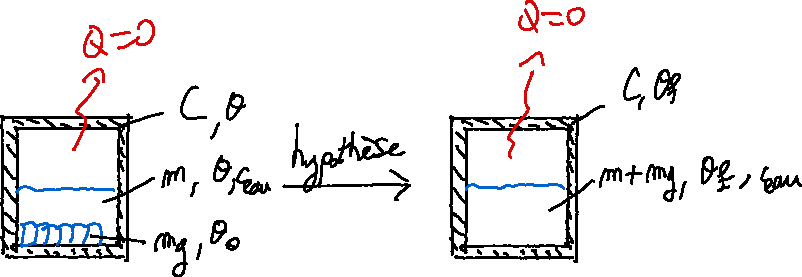
\includegraphics[scale=1]{calo_A}
	\end{center}
	\textbf{Hypothèse}~: on suppose que toute la glace a fondu. Dans ce cas, comme
	la transformation est isobare et que le calorimètre est calorifugé, on a
	\begin{align*}
		\Delta{H}\ind{tot}
		      & = Q = 0
		\\\Lra
		0
		      & =
		\Delta{H}\ind{calo} + \Delta{H}\ind{eau} + \Delta{H}\ind{glace}
		\\\beforetext{Or,}
		\Delta{H}\ind{calo}
		      & = C (T_f-T)
		\\
		\Delta{H}\ind{eau}
		      & = mc\ind{eau} (T_f-T)
		\\
		\Delta{H}\ind{glace}
		      & = m_g c\ind{eau} (T_f-T_0) + m_g \Delta{h}\ind{fus}
		\\\Lra
		(C + mc\ind{eau} + m_fc\ind{eau})T_f
		      & =
		(C + mc\ind{eau})T + m_gc\ind{eau}(T_f-T_0) - m_g\Delta{h}\ind{fus}
		\\\Lra
		\Aboxed{
		T_f   & =
			\frac{(C + mc\ind{eau})T + m_gc\ind{eau}(T_f-T_0) - m_g\Delta{h}\ind{fus}}
			{C + mc\ind{eau} + m_fc\ind{eau}}
		}
		\qav
		\left\{
		\begin{array}{rcl}
			\th                & = & \SI{18}{\degreeCelsius}
			\\
			\th_0              & = & \SI{0}{\degreeCelsius}
			\\
			C                  & = & \SI{150}{J.K^{-1}}
			\\
			m                  & = & \SI{100e-3}{kg}
			\\
			m_g                & = & \SI{25e-3}{kg}
			\\
			c\ind{eau}         & = & \SI{4.185e3}{J.K^{-1}.kg^{-1}}
			\\
			\Delta{h}\ind{fus} & = & \SI{335e3}{J.K^{-1}.kg^{-1}}
		\end{array}
		\right.
		\\
		\makebox[0pt][l]{$\phantom{\AN}\xul{\phantom{\th_f = \SI{2.76}{\degreeCelsius}}}$}
		\AN
		\th_f & = \SI{2.76}{\degreeCelsius}
	\end{align*}
	Ce qui est cohérent avec l'hypothèse.
}%

\QR{%
	Calculer la température d'équilibre pour $C = \SI{246}{J.K^{-1}}$ et $m_g =
		\SI{50}{g}$. Quelle proportion de glace a fondu~?
}{%
	Même expérience mais $C$ et $m_g$ changent. En appliquant la même formule, on
	obtient $\th_f = \SI{-5.5}{\degreeCelsius}$~! C'est incohérent avec
	l'hypothèse. On la reformule, en supposant un \textbf{équilibre diphasé
		glace/eau}. La température doit alors être $T_f = T_0$. On appelle $x$ la
	fraction d'eau qui a gelé. Nouveau schéma~:
	\begin{center}
		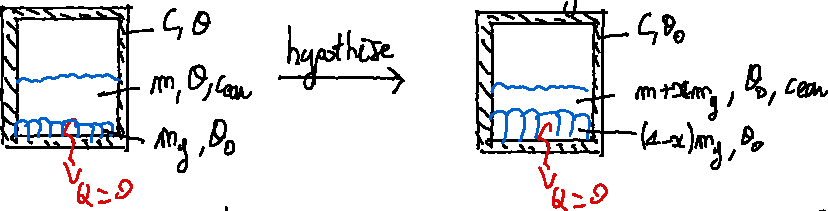
\includegraphics[scale=1]{calo_B}
	\end{center}
	Dans ce cas, l'eau et le calorimètre refroidissent jusqu'à
	$\SI{0}{\degreeCelsius}$, et une fraction $x$ de la glace fond. Ainsi,
	\begin{align*}
		\Delta{H}\ind{calo}  & = C (T_f - T)
		\\
		\Delta{H}\ind{eau}   & = mc\ind{eau} (T_0 - T)
		\\
		\Delta{H}\ind{glace} & = xm_g\Delta{h}\ind{fus}
		\\\beforetext{Avec $\Delta{H}\ind{tot} = 0$,}
		0
		                     & =
		(C+mc\ind{eau})(T_0 - T) + xm_g\Delta{h}\ind{fus}
		\\\Lra
		\Aboxed{
		x                    & = \frac{(C+mc\ind{eau})(T - T_0)}{m_g\Delta{h}\ind{fus}}
		}
		\qav
		\left\{
		\begin{array}{rcl}
			C   & = & \SI{245}{J.K^{-1}}
			\\
			m_g & = & \SI{50e-3}{kg}
		\end{array}
		\right.                                                                         \\
		\makebox[0pt][l]{$\phantom{\AN}\xul{\phantom{x = \num{0.71}}}$}
		\AN
		x                    & = \num{0.71}
	\end{align*}
	Autrement dit, \textbf{\num{71}\% de la glace a fondu}.
}%

\end{document}
